\chapter{Desenvolvimento do projeto}
\label{chap:fundteor}
%--------- NEW SECTION ----------------------
 Nesta seção será descrito o procedimento utilizado para construção inicial do robô Walker, incluindo as fases conceitual e design.  Será apresentado a ideação do projeto, especificações e as funcionalidades.

\section{Descrição}
 O Walker é um robô bípede, ou seja, um robô que se desloca sobre dois pés. Este robô deve ser capaz de se locomover e desviar de obstáculos em um determinado ambiente. Além disso, o Walker deve realizar um desafio, que consiste em navegar de forma autônoma, se localizar por meio de tags e encontrar um determinado objeto.

%conferir se precisa de requisitos do cliente
\subsection{Requisitos do cliente}
 O cliente definiu certos requisitos quanto à operação e  às características do robô:
 \begin{itemize}
    \item Operar em uma área de 2x1,5m;
    \item Possuir uma altura de aproximadamente 30 cm;
    \item Ser capaz de operar por, no mínimo 20 minutos;
    \item Ser capaz de desviar de obstáculos;
 \end{itemize}
\subsection{Arquitetura Geral}
 A arquitetura geral, apresentada na Figura \ref{fig:Arquitetura geral}, relaciona de modo geral a interface do usuário, com a central de gerenciamento do sistema e com a interface com hardware. Neste contexto, a interface do usuário representa o contato direto com o usuário por meio de um botão \textit{on/off}, um \textit{joystick} e por acesso remoto, através de um computador devidamente conectado.

 \begin{figure} [h!]	
    \centering

    \caption{Arquitetura Geral}
    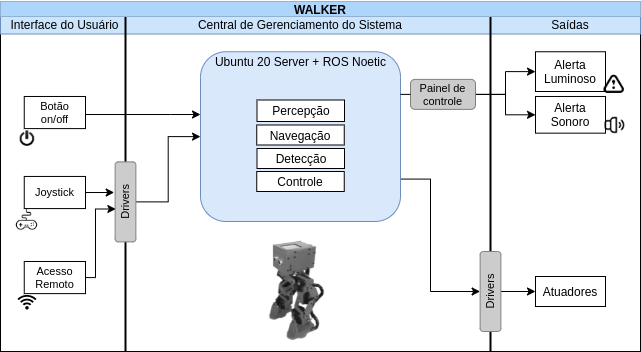
\includegraphics[width=0.8\textwidth]{general_architecture}
    \caption*{Fonte: Autoria própria.}
    \label{fig:Arquitetura geral}
\end{figure}	

Para a central de gerenciamento do sistema utilizou-se o sistema operacional \textit{Ubuntu} 20.04 junto ao framework de robótica ROS \textit{Noetic}. Neste cojunto se encontram as principais funcionalidades do robô: percepção, navegação, detecção e controle. Por fim, no conjunto de saídas estão os atuadores e os alertas sonoro e luminoso.

\subsection{Requisitos técnicos}

%desdobramento da função qualidade
\subsection{Quality Function Deployment}

%----------------------------------------------------------

%--------- NEW SECTION ----------------------
\section{Assunto 1}
\label{sec:ass1}
\lipsum[1]



%---------------picture------------------------------------
% \begin{figure}
%     \centering
%     \subfigure[Figure A]{\label{fig:a}\includegraphics[width=60mm]{./lq}}
%     \subfigure[Figure B]{\label{fig:b}\includegraphics[width=60mm]{./lq}}
%     \subfigure[Figure C]{\label{fig:c}\includegraphics[width=\textwidth]{./lq}}
%     \caption{Three simple graphs}
%     \label{fig:three graphs}
% \end{figure}
%----------------------------------------------------------

\begin{figure}
    \centering
    \begin{subfigure}[b]{0.3\textwidth}
        \centering
        \includegraphics[width=\textwidth]{./lq}
        \caption{$y=x$}
        \label{fig:y equals x}
    \end{subfigure}
    \hfill
    \begin{subfigure}[b]{0.3\textwidth}
        \centering
        \includegraphics[width=\textwidth]{./lq}
        \caption{$y=3sinx$}
        \label{fig:three sin x}
    \end{subfigure}
    \hfill
    \begin{subfigure}[b]{0.3\textwidth}
        \centering
        \includegraphics[width=\textwidth]{./lq}
        \caption{$y=5/x$}
        \label{fig:five over x}
    \end{subfigure}
       \caption{Three simple graphs}
       \label{fig:three graphs}
\end{figure}


%--------- NEW SECTION ----------------------
\section{Assunto 2}
\label{sec:ass2}
flkjasdlkfjasdlkfjs

\begin{table}[h]
    \begin{subtable}[h]{0.45\textwidth}
        \centering
        \begin{tabular}{l | l | l}
        Day & Max Temp & Min Temp \\
        \hline \hline
        Mon & 20 & 13\\
        Tue & 22 & 14\\
        Wed & 23 & 12\\
        Thurs & 25 & 13\\
        Fri & 18 & 7\\
        Sat & 15 & 13\\
        Sun & 20 & 13
       \end{tabular}
       \caption{First Week}
       \label{tab:week1}
    \end{subtable}
    \hfill
    \begin{subtable}[h]{0.45\textwidth}
        \centering
        \begin{tabular}{l | l | l}
        Day & Max Temp & Min Temp \\
        \hline \hline
        Mon & 17 & 11\\
        Tue & 16 & 10\\
        Wed & 14 & 8\\
        Thurs & 12 & 5\\
        Fri & 15 & 7\\
        Sat & 16 & 12\\
        Sun & 15 & 9
        \end{tabular}
        \caption{Second Week}
        \label{tab:week2}
     \end{subtable}
     \caption{Max and min temps recorded in the first two weeks of July}
     \label{tab:temps}
\end{table}